\documentclass[a4paper,10pt]{article}
\usepackage[french]{babel}
\usepackage[utf8]{inputenc}
\usepackage[left=2.5cm,top=2cm,right=2.5cm,nohead,nofoot]{geometry}
\usepackage{url}
\usepackage{graphicx}
\usepackage{hyperref}
\usepackage{listings}
\usepackage{amsmath}

\linespread{1.1}

\usepackage{xcolor}
\usepackage{inconsolata}

\begin{document}

\lstset{
    pad\mathcal{R}o
    basicstyle=\ttfamily\small,
    numberstyle=\footnotesize,
    numbers=left,
    backgroundcolor=\color{gray!10},
    frame=single,
    tabsize=2,
    rulecolor=\color{black!30},
    title=\lstname,
    escapeinside={\%*}{*)},
    breaklines=true,
    breakatwhitespace=true,
    framextopmargin=2pt,
    framexbottommargin=2pt,
    extendedchars=false,
    inputencoding=utf8,
    literate={à}{{\`a}}1 {è}{{\`e}}1 {é}{{\'e}}1,
}

\begin{titlepage}
\begin{center}
\textbf{\textsc{UNIVERSIT\'E LIBRE DE BRUXELLES}}\\
%\textbf{\textsc{Faculté des Sciences}}\\
%\textbf{\textsc{Département d'Informatique}}
\vfill{}\vfill{}
\begin{center}{\Huge Rapport : HORECA}\end{center}{\Huge \par}
\begin{center}{\large Thomas Perale (408160)}\end{center}{\Huge \par}
\vfill{}\vfill{} \vfill{}
\begin{flushleft}{\large \textbf{INFO-H-303 Base de données}}\hfill{Esteban Zimányi, Michaël Waumans}\end{flushleft}{\large\par}
\vfill{}\vfill{}\enlargethispage{3cm}
\textbf{Année académique 2015-2016}
\end{center}
\end{titlepage}

%\begin{abstract}
%Ce rapport présente ...
%\end{abstract}


\tableofcontents

\pagebreak


\section{Diagramme entité association}
\subsection{Diagramme}
\begin{figure}[hbt]
    \centering
    \includegraphics[scale=0.4]{bdd.png}
    \caption{Diagramme entité association}
\end{figure}
\subsection{Contraintes}
Les contraintes sont les suivantes :
\begin{itemize}
  \item Le couple (Longitude, Latitude) est unique.
  \item La longitude et la latitude doivent être comris entre -180 et 180.
  \item Le nom d'utilisateur est unique.
  \item L'email d'utilisateur est unique.
  \item Pour les commentaire, le couple (IdUtilisateur, date) est unique. Donc
      un même utilisateur ne peut pas écrire deux commentaires en même temps.
  \item Pour les labels, le triplet : (Label, IdArticle, IdUtilisateur) est
      unique, ça veut dire qu'une personne ne peut pas ajouter deux fois le
      même label.
  \item Le nombre d'étoile (commentaire et hotel), doit être compris entre 1 et 5.
  \item Les ID des hotels/bars/restaurants référencent ceux de la table
      établissement, chaque établissement est soit un hotel, soit un bar, soit
      un restaurant, il ne peut pas être deux type d'établissement en même
      temps.
  \item La Date de création d'un établissement doit précéder celle de ses commentaires.
  \item La Date d'enregistrement d'un admin doit précéder celle de création d'un établissement par celui-ci.
  \item La Date d'enregistrement d'un utilisateur doit être antérieur à celle où il a écrit un commentaire.
\end{itemize}



\section{Modèle relationnel}
\subsection{Modèle}

\begin{description}
\item[] \textbf{Utilisateur}(\underline{Id}, Email, MotDePasse, DateEnregistrement, Admin(0, 1))
    \begin{description}
        \item[] Utilisateur.Admin indique si l'utilisateur est un admin ou non.
    \end{description}

\item[] \textbf{Etablissement}(\underline{Id}, Nom, Adresse.Rue,
    Adresse.Numéro, Adresse.CodePostal, Adresse.Localité, Coordonnée.Latitude,
    Coordonnée.Longitude, Téléphone, Site, DateCreation, Creator)
    \begin{description}
        \item[] Etablissement.Creator réfèrence Utilisateur.Id.
    \end{description}

\item[] \textbf{Restaurant}(\underline{Id}, Prix, Places, AEmporter, Livraison, horaire)
    \begin{description}
        \item[] Restaurant.Id réfèrence Etablissement.Id.
    \end{description}

\item[] \textbf{Bar}(\underline{Id}, Fumeur, Snacks)
    \begin{description}
        \item[] Bar.Id réfèrence Etablissement.Id.
    \end{description}

\item[] \textbf{Hotel}(\underline{Id}, NombreEtoile, NombreChambre, Prix)
    \begin{description}
        \item[] Hotel.Id réfèrence Etablissement.Id.
    \end{description}

\item[] \textbf{Commentaire}(\underline{Id}, Commentaire, NombreEtoile, Date,
    Image, IdArticle, IdUtilisateur)
    \begin{description}
        \item[] Commentaire.IdArticle réfèrence Etablissement.Id.
        \item[] Commentaire.IdUtilisateur réfèrence Utilisateur.Id.
    \end{description}

\item[] \textbf{Label}(\underline{Id}, Label, IdArticle, IdUtilisateur)
    \begin{description}
        \item[] Commentaire.IdArticle réfèrence Etablissement.Id.
        \item[] Commentaire.IdUtilisateur réfèrence Utilisateur.Id.
    \end{description}
\end{description}

\subsection{Contraintes}

\begin{itemize}
    \item On doit d'abord créer l'établissement avant de créer sa
        spécialisation (restaurant, bar, hotel) de manière à pouvoir
        référencer cet établissement.
\end{itemize}

\section{Hypothèses}
Les utilisateur "admin" sont encodé directement dans la base de donnée.
\newline

Il est marqué dans l'énoncé :
\begin{quote}
    Les utilisateurs peuvent commenter plusieurs fois le même
    établissement à des dates différentes.
\end{quote}
Les dates seront stocké dans ma base de donnée sous forme de \emph{timestamp},
dés lors un utilisateur ne pourra pas envoyer deux message lors de la même seconde.
\newline

Un administrateur peut modifier un établissement, mais j'ai décidé de ne pas
stocker les dates de modification mais seulement celle de création.
\newline

Les adresses mails ainsi que les mot de passes des \emph{Utilisateur} qui nous
sont fournis dans le fichier \emph{Data.zip} peuvent être choisis.

\section{Justification}

J'ai décidé pour la généralisation des établissements d'hériter les clées
principales qui sont dans établissement. De cette manière j'évite de devoir
redéclarer à chaque fois dans chaques table spécialisée (hotel, restaurant ou
bar) les mêmes données. De plus la recherche de d'établissement par nom est
rendue plus simple. \newline

Pour le généralistion des utilisateurs j'ai décidé d'ajouter une colonne
"Admin" dans la table utilisateur pour permettre de savoir si un utilisateur
est admin ou non. \newline

En ce qui concerne les \emph{labels} j'ai décidé de mettre l'\emph{ID} de
l'utilisateur dans une des colonnes, de cette façon on sait facilement savoir
si une personne a déjà ajouté un certain label ou non.

\section{Script SQL DDL}
    \lstinputlisting[language=SQL]{../db/create.sql}

    \pagebreak

\section{Requêtes}
\subsection{Tous les Utilisateurs qui apprécient au moins 3 établissements que
l'utilisateur \emph{Brenda} apprécie.}
    Les résultats de cette requête sont visible dans l'application à la page
    \emph{/user/Brenda}.
    \lstinputlisting[language=SQL]{../db/1.sql}
\subsubsection{Algèbre relationnelle}
\begin{align}
    \Pi_{c1.username}comments \sigma_{count(c1.username)>=3}
    \\\bowtie_{'Brenda'=c2.username AND
    c1.establishment\_id=c2.establishment\_id AND c2.rating>=4 AND
    c1.rating>=4}
\end{align}

\subsubsection{Calcul relationnel}
\begin{align}
    \{ c1.username | comments(c1) \wedge \\
    \exists c2 ( comments(c2) \\
        \wedge c2.username='Brenda' \\
        \wedge c1.establishment\_id=c2.establishment\_id \\
        \wedge c1.rating>=4 \wedge c2.rating>=4 \\
        \wedge c1.username!='Brenda') \}
\end{align}

% ---------------------------------------------------------------------------

\subsection{Tous les établissements qu'apprécie au moins un utilisateur qui
apprécie tous les établissements que \emph{Brenda} apprécie.}
    \lstinputlisting[language=SQL]{../db/2.sql}

\subsection{Tous les établissements pour lesquels il y a au plus un
commentaire.}
    Les résultats de cette requête sont visible dans l'application à la page
    \emph{/establishments/discover}
    \lstinputlisting[language=SQL]{../db/3.sql}

\subsubsection{Algèbre relationnelle}
    \begin{align}
        \Pi_{c.establishment_id}comments \sigma_{count(c.establishment_id)<=1}\Pi_{c.establishment_id}
    \end{align}

\subsubsection{Calcul relationnel}
\begin{align}
    \{ c.establishment\_id | comments(c) \wedge \\
    \exists (c.username_1, c.username_2) \\
    \wedge (c.username_1 != c.username_2) \}
\end{align}

% ---------------------------------------------------------------------------

\subsection{La liste des administrateurs n'ayant pas commenté tous les
établissements qu'ils ont crées.}
    \lstinputlisting[language=SQL]{../db/4.sql}

\subsubsection{Algèbre relationnelle}
\begin{align}
    \Pi_{a.username}\ account \\
        \sigma_{a.admin\ AND \\
        \nexists_{(\Pi_{e.created\_by}\ establishment) \\
        \bowtie_{e.id=c.establishment\_id \ AND \ e.created\_by!=c.username}} \\
        \Pi_{c.establishment\_id}}
\end{align}

\subsubsection{Calcul relationnel}
\begin{align}
    \{ a.username | account(a) \wedge \\
    \exists a(a.admin=1) \wedge \\
    \neg (e.created\_by | establishment(e) \\
        \exists c(comments(c) \wedge \\
        e.id=c.establishment\_id \wedge e.created_by!=c.username) \\
    ) \}
\end{align}

% ---------------------------------------------------------------------------

\subsection{La liste des établissements ayant au minimum trois commentaires,
classée selon la moyenne des scores attribués.}
    Les résultats de cette requête sont visible dans l'application à la page
    \emph{/establishments/ratings}
    \lstinputlisting[language=SQL]{../db/5.sql}

\subsubsection{Algèbre relationnelle}
\begin{align}
    \Gamma_{AVG(c.rating)}\Pi_{AVG(c.rating), c.establishment_id}comments \sigma_{count(c.establishment_id)>=3}\Pi_{c.establishment_id}
\end{align}

\subsubsection{Calcul relationnel}
\begin{align}
    \{ c.establishment\_id | comments(c) \wedge \\
    \exists c_1, c_2, c_3 ( \\
        c_1.establishment\_id = c_2.establishment\_id = c_3.establishment\_id \\
        \wedge c_1.username != c_2.username != c_3.username
    ) \}
\end{align}

% ---------------------------------------------------------------------------

\subsection{La liste des labels étant appliqués à au moins 5 établissements,
classée selon la moyenne des scores des établissements ayant ce label.}
    Les résultats de cette requête sont visible dans l'application à la page
    \emph{/establishments/label/\ldots}
    \lstinputlisting[language=SQL]{../db/6.sql}

\subsubsection{Algèbre relationnelle}
    \begin{align}
        \Gamma_{AVG(c.rating)}\Pi_{AVG(c.rating), l.name}label \sigma_{count(DISTINCT l.establishment_id)>=5}\Pi_{l.name}
        \\\bowtie_{c.establishment_id=l.establishment_id}
    \end{align}

\subsubsection{Calcul relationnel}
\begin{align}
    \{ l.name | label(l) \wedge \\
    \exists l_1, l_2, l_3, l_4, l_5 ( \\
        l_1.establishment\_id != l_2.establishment\_id != l_3.establishment\_id != l_4.establishment\_id != l_5.establishment\_id\wedge \\
        l_1.name = l_2.name = l_3.name = l_4.name = l_5.name \\
    ) \}
\end{align}

% ---------------------------------------------------------------------------

\section{Implémentation}
\subsection{Language et libraires}
\begin{itemize}
    \item \emph{Express.js} comme frameword web pour le language \emph{node.js}.
    \item \emph{Handlebars.js} comme moteur de template pour \emph{express.js}.
    \item \emph{Bootstrap} et \emph{jQuery} comme framework de frontend.
    \item \emph{SQLite3} comme moteur de base de donnée.
\end{itemize}

\subsection{Script d'insértion de données}
    \lstinputlisting[language=python]{../init.py}
    \pagebreak

\subsection{Instruction d'installation de l'application}
À la racine du projet.
\begin{lstlisting}
make
npm install
node index.js
\end{lstlisting}

\subsection{Liaison avec la base de donnée.}
L'accès par l'application à la base de donnée se fait par l'ensemble des
fonctions stockées dans le dossier \emph{./db/}.
\begin{itemize}
    \item [database\_utils.js] Ensemble de fonctions qui intéragissent avec tout les
        établissements.
    \item [restaurant\_db\_utils.js] Ensemble de fonctions qui intéragissent
        avec les restaurants.
    \item [bar\_db\_utils.js] Ensemble de fonctions qui intéragissent avec les
        bars.
    \item [hotel\_db\_utils.js] Ensemble de fonctions qui intéragissent avec
        les hotels.
    \item [label\_db\_utils.js] Ensemble de fonctions qui intéragissent avec
        les labels.
    \item [comment\_utils.js] Ensemble de fonctions qui intéragissent avec
        les commentaires.
\end{itemize}

\section{Application}
\subsection{Page principale.}
La page principale est la première page de l'application que l'utilisateur va
voir. Dans cette page, plusieurs chose sont déjà possible :

\begin{itemize}
    \item S'inscrire
    \item Se connecter
    \item Choisir parmis une selection d'établissement pris au hasard.
    \item Acceder à une selection d'établissement plus spécifique.
    \item Une carte des établissements qui sont sur le site.
\end{itemize}

\begin{figure}[hbt]
  \centering
  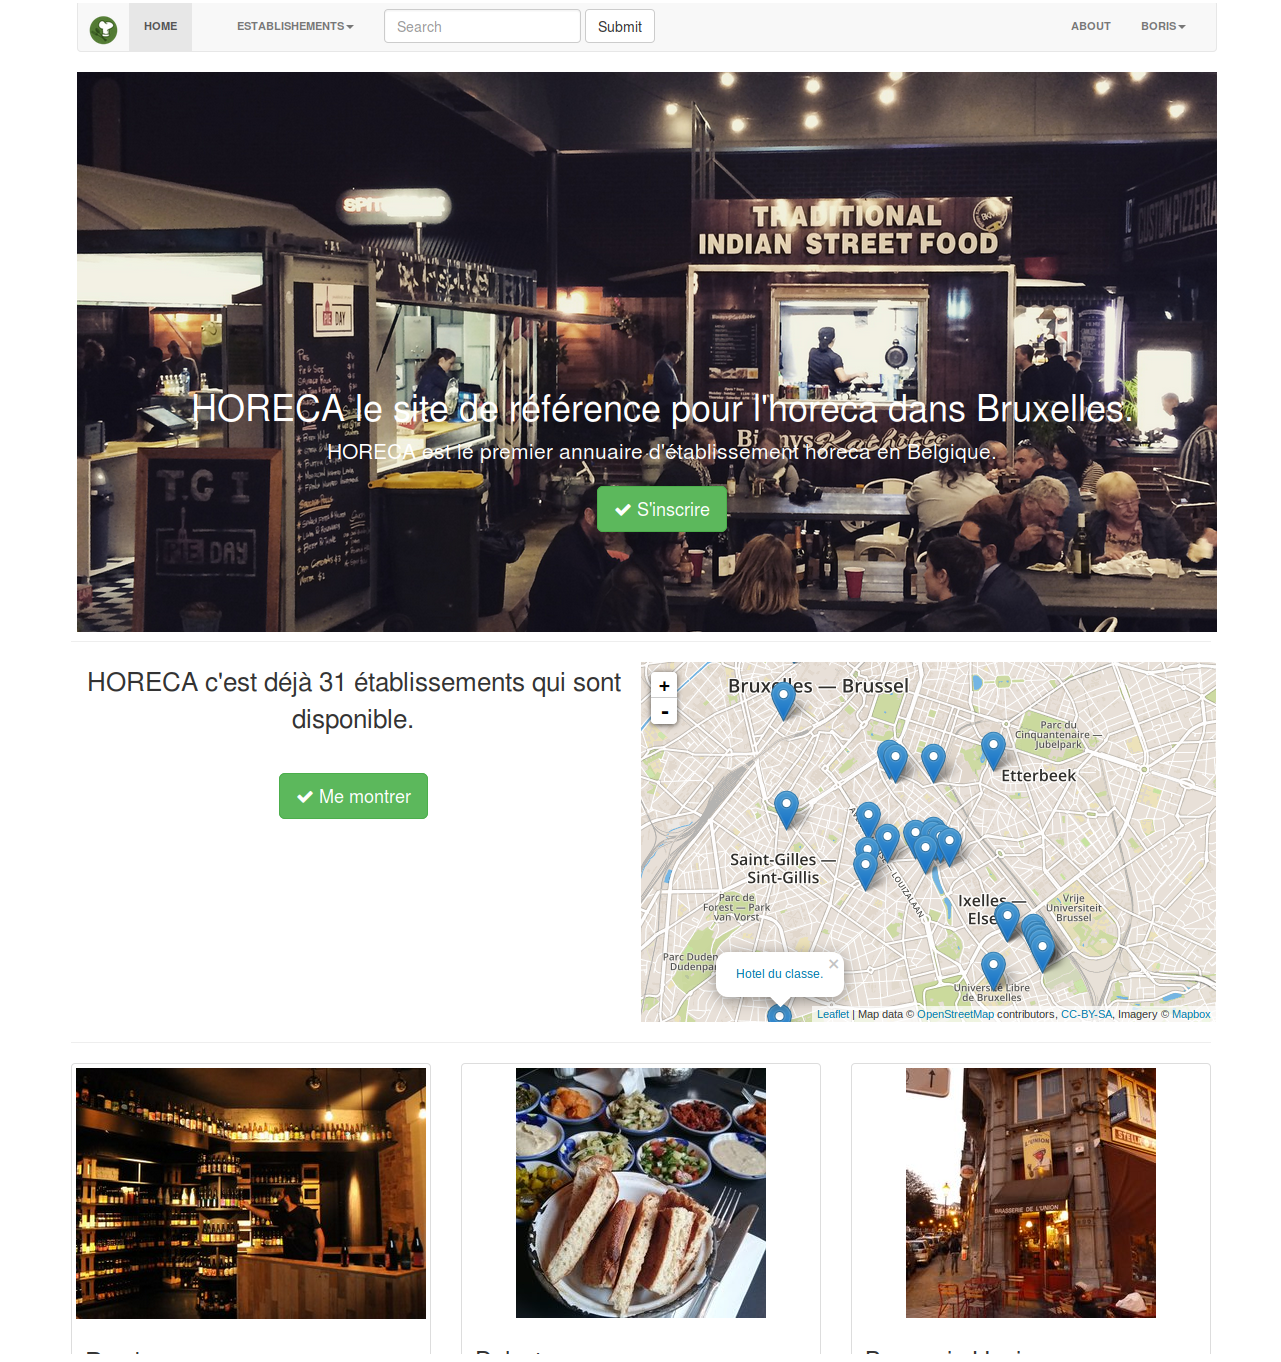
\includegraphics[scale=0.2]{./images/main.png}
  \caption{Page principale.}
\end{figure}

\subsection{Établissements}
La page des établissements donne à l'utilisateur un coup d'ouil sur ses
caractéristiques propres. Mais c'est aussi un lieu pour les utilisateurs de
donner leur avis sur l'établissement et de le classer dans des catégories.
Chaques commentaire qu'un utilisateur laisse peut être mis en avant par un
système de vote individuel au commentaire, de cette façon les commentaires qui
sont malhonnêtes selon les utilisateurs sont visibles.

\begin{figure}[hbt]
  \centering
  \includegraphics[scale=0.2]{./images/establishment.png}
  \caption{Page principale.}
\end{figure}

\subsection{Utilisateur}
\begin{figure}[hbt]
  \centering
  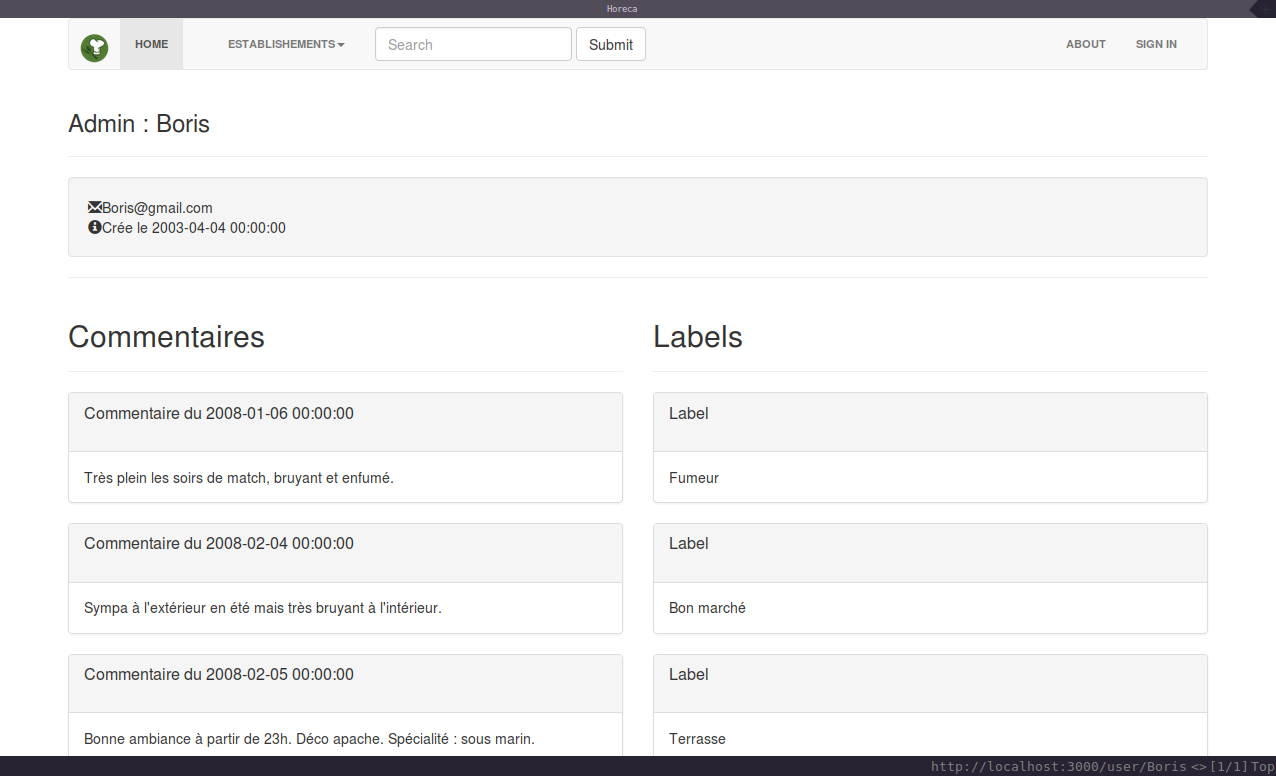
\includegraphics[scale=0.2]{./images/user.png}
  \caption{Page utilisateur.}
\end{figure}

\section{Apports personnels}
\subsection{Site adapté aux mobiles}
    Pour que l'application soit adaptée au type de consommation actuelle, elle
    a été crée dans l'idée de pouvoir aussi bien est facile d'utilisation sur
    ordinateur que sur mobile.

    \begin{figure}[hbt]
        \centering
        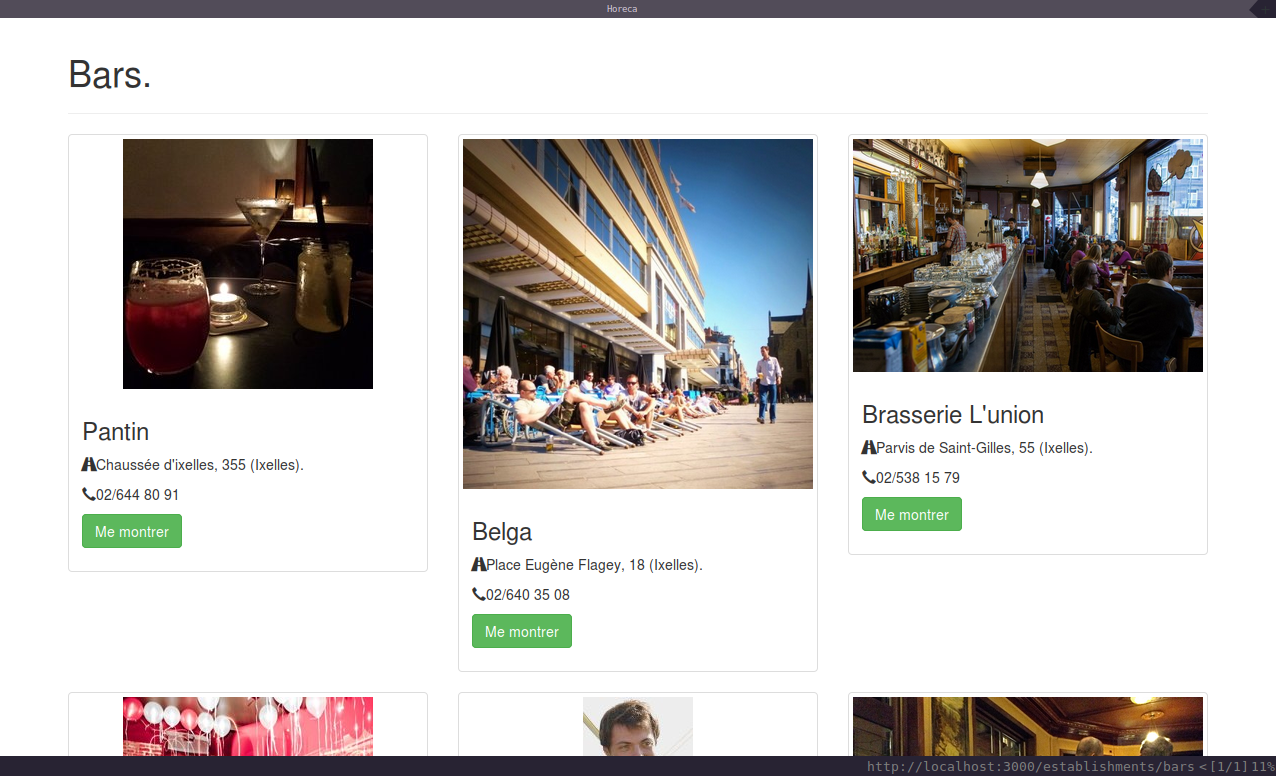
\includegraphics[scale=0.2]{./images/responsive.png}
        \caption{Site responsive.}
    \end{figure}

\subsection{Utilisateur administrateur}
    Des comptes administrateur sont à disposition pour pouvoire gèrer les
    publications, si celle-ci doivent être changer, ou pour faire un travail de
    modération dans les commentaires ou les labels.
    Un administrateur a le pouvoir de :
    \begin{itemize}
        \item Supprimer un commentaire.
        \item Supprimer un label.
        \item Supprimer un établissement.
        \item Supprimer un utilisateur.
        \item Ajouter d'autres utilisateur au poste d'adminisatrateur.
        \item Créer des restaurants.
        \item Créer des hotels.
        \item Créer des bars.
        \item Modifier les données des établissements.
    \end{itemize}
\subsection{Localisation des restaurants sur une carte}
    Afin de permettre de pouvoir directement voir l'emplacement des
    établissements sur une l'application intêgre des cartes pour visualiser
    l'emplacement de l'établissement \emph{HORECA}. Celles-ci sont intégrées à
    la page web à l'aide d'une bibliothèque Javascript, Leaflet.
    En plus de montrer l'emplacement sur une carte celles-ci montre aussi un
    rapide aperçu des caractéristiques de l'établissement.

    \begin{figure}[hbt]
        \centering
        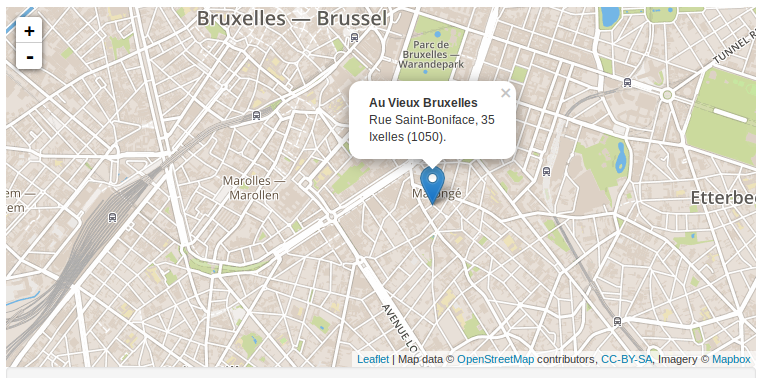
\includegraphics[scale=0.4]{./images/card.png}
        \caption{Établissement indiqué sur une carte.}
    \end{figure}

\subsection{Géolocalisation sur la carte}
    En plus de montrer la localisation des restaurants, l'application permet
    de pouvoir se géolocaliser sur la carte, par apport aux établissements.
    \newline
    Cette fonctionnalitée est d'autant plus la bienvenue que l'application est
    adaptée aux téléphones mobiles.

    \begin{figure}[hbt]
        \centering
        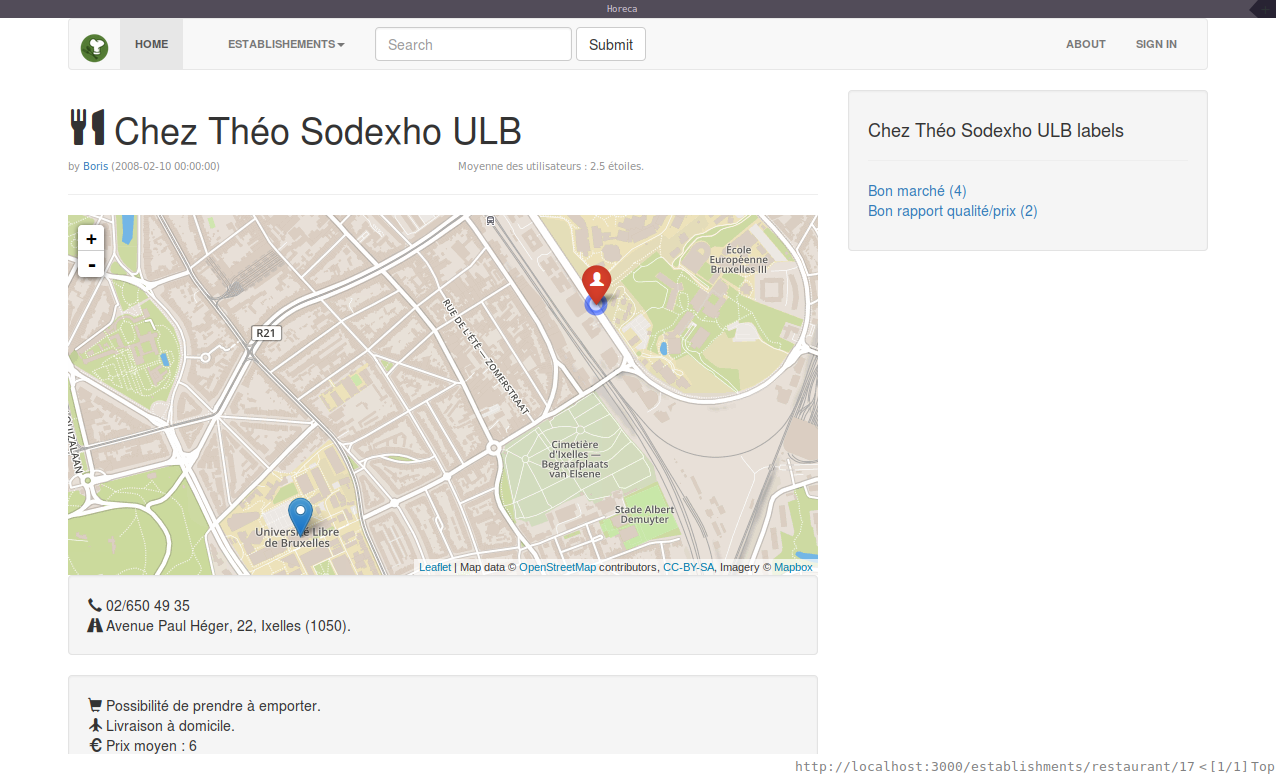
\includegraphics[scale=0.4]{./images/geolocalisation.png}
        \caption{Un marqueur indique l'endroit où l'on se trouve.}
    \end{figure}


\subsection{Gestion des photos}
    L'application gère le stockage d'image dans la base de donnée.
    Chaques utilisateur inscrit sur le site peuvent dés lors écrire un
    commentaire dans la section adaptée accompagné d'une photo de
    l'établissement visité par exemple. \newline
    Quant aux utilisateurs dit \emph{administrateur}, ils peuvent modifier
    la photo de l'établissement pour que chaques visiteur aie un aperçu de
    l'apparence de l'établissement. \newline
    De plus la gestion de ces photos permet de les visionner de manière
    comfortable à l'aide du module enhance.js. En effet celui-ci permet de voir
    une photo \emph{en grand}, sans devoir changer de page.

    \begin{figure}[hbt]
        \centering
        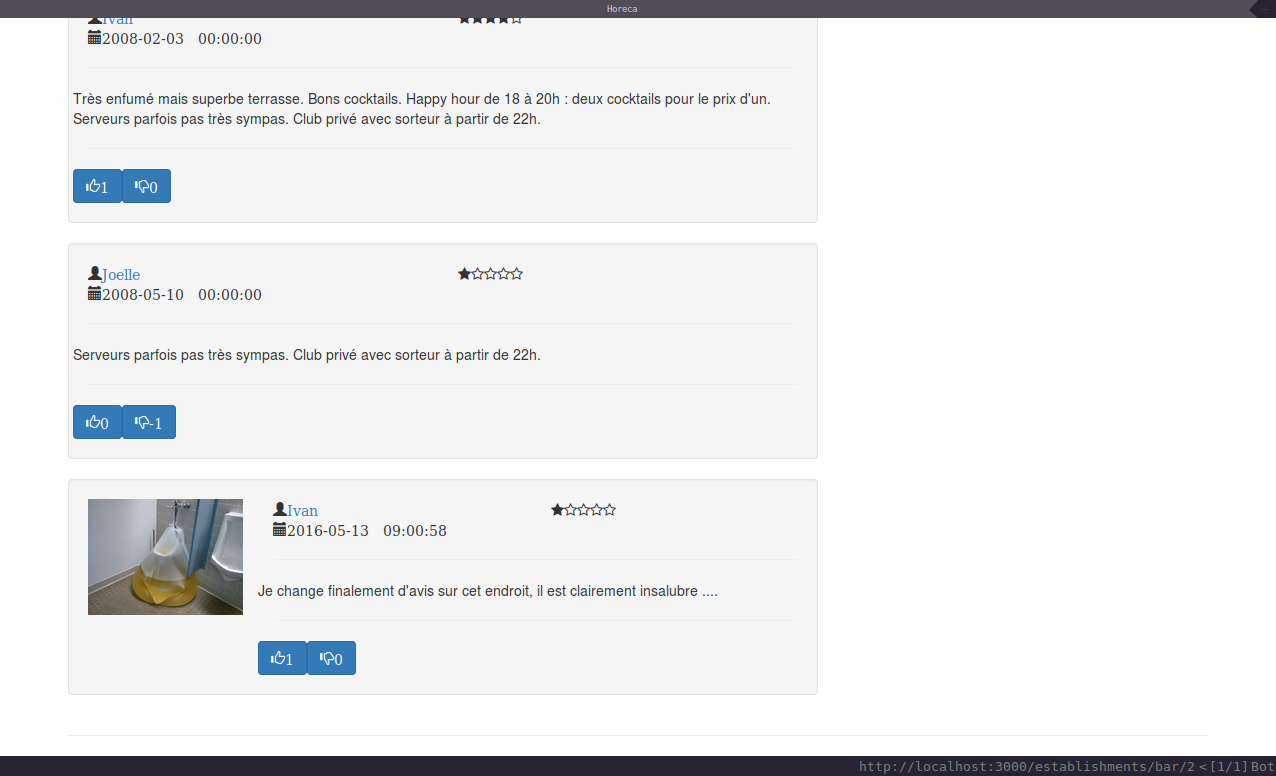
\includegraphics[scale=0.3]{./images/picture.png}
        \caption{Ici un commentaire accompagné d'une photo.}
    \end{figure}

\subsection{Recherche de label similaire.}
    Pour permettre aux visiteurs de trouver des établissements avec des
    contraintes spécifiques, l'application lie tout les labels de chaques
    établissements. Un visiteurs peut dés lors retrouver tout les
    établissements qui possède le label de son choix, comme par exemple
    \emph{Fumeur}.

    \begin{figure}[hbt]
        \centering
        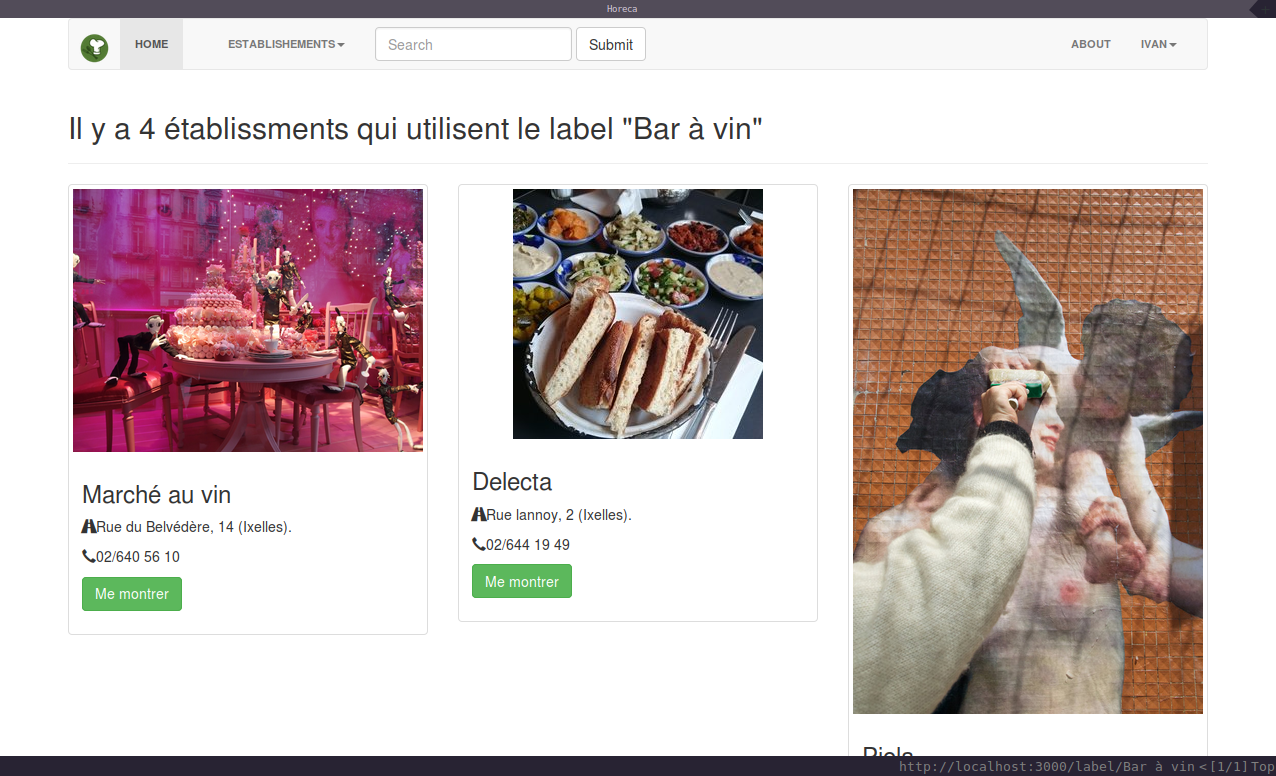
\includegraphics[scale=0.3]{./images/label.png}
        \caption{Page regroupant les établissements sous le label "Bar à vin".}
    \end{figure}



\subsection{Vote dans les commentaires}
    Un système de vote individuel à chaques commentaire est mit en place pour
    que chaque utilisateur inscript aie le droit de juger des commentaires
    qui selon lui ne sont pas raisonnable ou inversément.

    \begin{figure}[hbt]
        \centering
        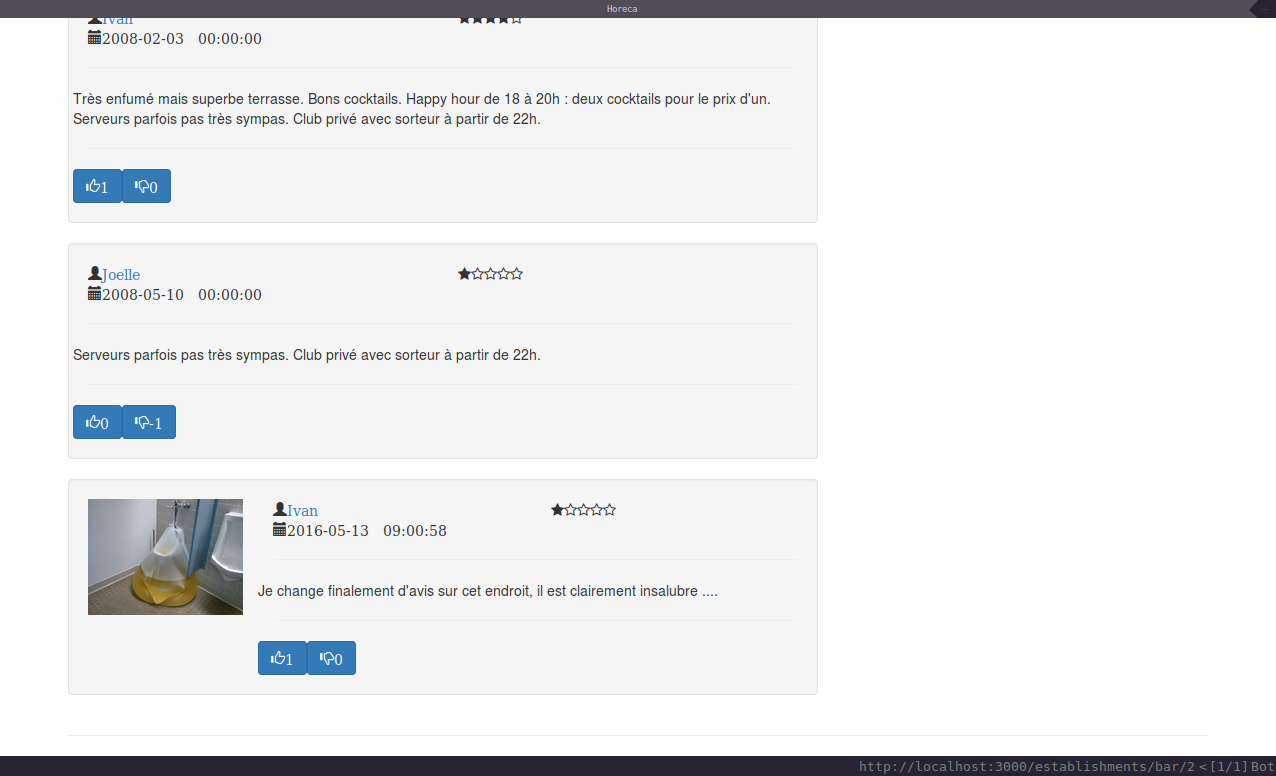
\includegraphics[scale=0.3]{./images/picture.png}
        \caption{Des votes en dessous de chaques commentaire.}
    \end{figure}


\end{document}
